\subsection{SEOSS evaluation with GPT 3.5 and GPT 4}  

Here we discuss our experience using the ChatGPT API for the Text-to-SQL task on the SEOSS dataset. We will provide a brief overview of the \ac{GPT} architecture and delve into the specifics of ChatGPT, emphasizing its capabilities and potential for addressing this particular challenge.
\subsubsection{GPT Architecture}

Generative Pre-trained Transformers (GPT) \cite{radford2018improving} represent the state-of-the-art in language modeling, being built upon the revolutionary Transformer architecture. This architecture has profoundly influenced the field of natural language processing due to its utilization of self-attention mechanisms. These mechanisms enable the parallel processing of sequences, leading to more efficient training and enhanced performance across a wide range of NLP tasks.

Inherently generative, GPT models are designed to create text based on the context they are given. They are pre-trained on vast quantities of textual data, which enables them to learn the underlying structure and patterns present in natural language. The pre-training phase consists of unsupervised learning using a masked language modeling objective. Following pre-training, GPT models can be fine-tuned for specific tasks, such as translation, summarization, or, as in our example, Text-to-SQL.

Prior to the introduction of GPT-4, OpenAI had developed three earlier GPT versions and had been refining GPT language models over an extended period. The first GPT model, launched in 2018, incorporated 117 million parameters. The next version, GPT-2, was released in 2019 and demonstrated a substantial increase, incorporating 1.5 billion parameters. GPT-3, which currently powers ChatGPT, made its debut in 2020 and operates with 175 billion parameters. OpenAI, however, has chosen not to reveal the number of parameters used in GPT-4 \cite{openai2023gpt4}.

Considering the consistent growth in parameter counts with each successive model, it is logical to assume that the most recent multimodal iteration features a higher number of parameters than its predecessor, GPT-3, which consists of 175 billion parameters. Also, some researchers have speculated that GPT-4 may have as many as 1 trillion parameters or more\cite{bubeck2023sparks}.

\subsubsection{ChatGPT}

\begin{figure}[H]
    \begin{AIbox}{Attention!}
        \parbox{1\textwidth}{
            Please note that the results in this section may be subject to change as ChatGPT continues to improve its system over time.
        }
    \end{AIbox}
\end{figure}


ChatGPT and \ac{LLM} models represent an evolution in language models tailored explicitly for conversational interfaces. These models exhibit a distinct behavior compared to older language models. While previous models operated on a text-in and text-out basis (accepting a prompt string and returning a completion to append to the prompt), GPT-3 and GPT-4 models follow a conversation-in and message-out approach \cite{bubeck2023sparks}. They expect input formatted in a chat-like transcript format and return a completion representing a model-generated message within the chat. This format is designed for multi-turn conversations but can also be effective in non-chat scenarios.
For our experiment with the SEOSS dataset, we utilized the ChatGPT API to submit natural language questions and retrieve generated SQL queries. The API allowed for the seamless integration of ChatGPT into our workflow and provided an efficient and effective means to process the dataset.
Throughout the evaluation, we observed that ChatGPT successfully generated accurate and syntactically correct SQL queries for a wide range of questions. The model excelled at handling complex queries and demonstrated a deep understanding of the underlying database schema.
However, there were instances where ChatGPT generated SQL queries that deviated from the desired output, particularly in edge cases and questions with ambiguous semantics. To mitigate this issue, we employed a combination of custom LLM prompts to ensure the generated queries met the required quality standards.

\subsubsection{Prompt Engineering}

Prompt Engineering is an emerging field focused on creating and refining prompts to enhance the performance of language models (LMs) across diverse applications and research areas. Mastering the art of prompt engineering allows researchers to gain deeper insights into the potential and boundaries of large language models (LLMs) while enabling them to augment LLMs' proficiency in handling typical and intricate tasks such as question answering and arithmetic reasoning. Additionally, developers employ prompt engineering to devise reliable and efficient prompting strategies that can seamlessly integrate with LLMs and other relevant tools. \cite{Saravia_Prompt_Engineering_Guide_2022}

Prompt engineering best practices encompass utilizing LLM APIs for various tasks, such as summarization, inference, text transformation, and expansion. The process of crafting effective prompts involves the systematic development of high-quality prompts to achieve optimal results in various tasks and applications.

\begin{figure}[H]
    \centering
    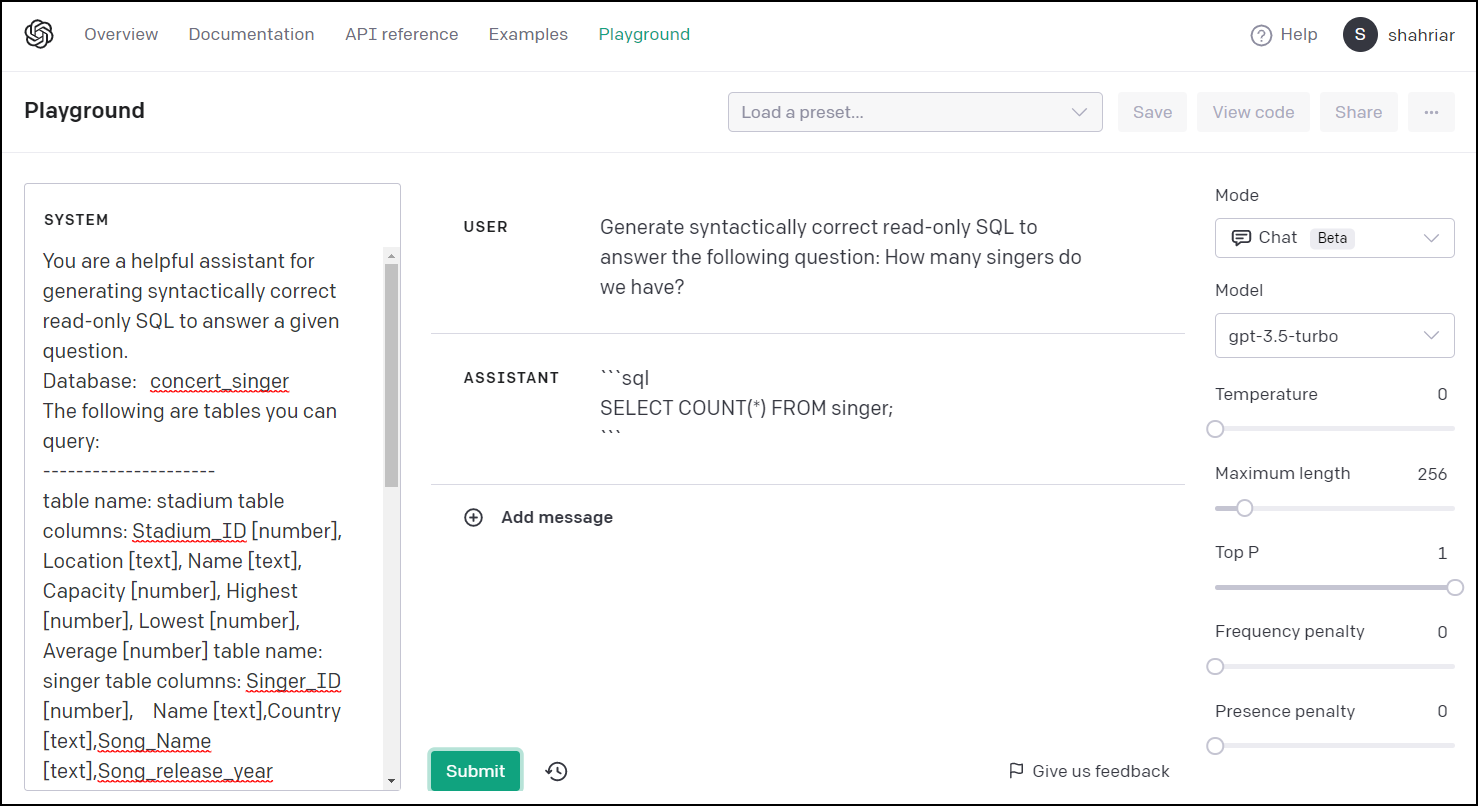
\includegraphics[width=0.9\textwidth]{pics/openai.png}
    \caption{OpenAI ChatGPT Prompting Portal}
    \label{fig:openai}
\end{figure}

OpenAI Playground shown in figure \ref{fig:openai} is a versatile development platform enabling users to explore and experiment with AI models such as the GPT-3 and GPT-4 series. This complimentary tool is designed to facilitate the development and testing of predictive language models using natural language processing techniques to comprehend user input text. The AI algorithm generates contextually appropriate and dynamic responses based on its vast training data.

Within the online Playground, researchers can choose between various AI model versions and adjust parameters such as Temperature, Maximum length, Top P, and Frequency and Presence penalties.

Temperature, ranging from 0 to 1, dictates the AI model's creativity. A lower temperature yields more predictable, fact-based responses, while a higher temperature produces more creative and random outputs. The default setting of 0.7 is recommended for most creative tasks.

Top P, on the other hand, is an alternative method to control output randomness and creativity. Tokens are organized and ranked according to their relevance to the prompt, and the "p" denotes probability. Adjusting the Top P value influences the range of available tokens.

The Playground also features two penalty functions to regulate repetition in the generated text: Frequency and Presence penalties. Frequency penalties minimize word repetition, while Presence penalties reduce the recurrence of specific topics. The penalty scale ranges from 0 to 2, with higher values indicating a lower likelihood of repeated tokens.

\subsubsubsection{Rules}

ChatGPT employs prompts to direct its response generation process \cite{white2023prompt}. 
To maximize the effectiveness of ChatGPT in various applications, it is essential to understand the art of crafting effective prompts. The following guidelines have been established to optimize the performance of ChatGPT in generating accurate, relevant, and context-aware responses:

\begin{enumerate}
    \item \textbf{Give ChatGPT an identity and intended audience}: By assigning a role or identity to ChatGPT (e.g., "You are a text-to-sql assistant, do... or As an assistant, do...") and specifying the target audience, the model can adopt a specific perspective or tone, providing tailored responses to the context.

    \item \textbf{Offer and give specific context}: Including relevant background information or context in the prompt helps the model generate more accurate and meaningful answers, particularly when dealing with complex or domain-specific queries.

    \item \textbf{Highlight information to include or exclude}: Clearly specifying what information should be incorporated or omitted in the response enables ChatGPT to generate responses that better align with user expectations (e.g. "Do not use any aliases").

    \item \textbf{Choose a relevant tone of voice and writing style}: Indicating the desired tone (e.g., formal, informal) or writing style (e.g., persuasive, explanatory) in the prompt can guide ChatGPT in producing responses that are more suitable for the specific application.

    \item \textbf{Give examples to base the response on}: Providing example responses can help ChatGPT understand the desired output format and style, allowing it to generate similar responses.

    \item \textbf{Specify response length}: Mentioning the required response length (e.g., "In 256 characters or less, do...") helps in obtaining outputs that conform to the desired word count or character limit. When we know the desired response length, with this rule we can also control the number of tokens generated by the model that will have a cost effect.

    \item \textbf{Clarity and specificity}: Crafting clear and concise prompts, along with avoiding ambiguous or vague questions, can significantly improve the quality of the generated responses. Easily by providing exact information and clear instructions to the model, we can get significantly better results.
\end{enumerate}

These guidelines, when employed systematically, can enhance the performance of ChatGPT in a wide range of natural language processing tasks. By iterative refining and experimenting with different prompt styles, we can achieve improved outcomes in our specific applications.

\subsubsubsection{Roles}

Prompts are input messages with an associated role, which can fall into one of three categories: system, user, or assistant. The role of the message's author supplies context for the conversation and influences the model's response. \cite{openai2023gpt4}

\begin{itemize}
    \item \textbf{System}: A high-level directive for the conversation, typically used to offer guidance or establish the context for the assistant.
    \item \textbf{User}: A message submitted by the user, usually in the form of a question or a request for the assistant to process.
    \item \textbf{Assistant}: The response produced by the assistant is based on the context provided by the system and user messages. The assistant processes the messages according to their order in the list and generates a response accordingly. Employing system instructions can effectively guide the assistant's behavior throughout the conversation. The assistant prompt is usually used to provide historical context for the conversation. 
\end{itemize}

Now we outline our approach to discovering the optimal prompt for text-to-SQL ChatGPT agents and present some preliminary results.
The initial step in identifying the best prompt involves defining a set of criteria to evaluate the quality and accuracy of the generated SQL commands.

Potential criteria include the syntactic correctness of the SQL commands (i.e., adherence to the rules and patterns of SQL syntax) and the semantic correctness of the SQL commands (i.e., alignment with the meaning and intent of the natural language queries).

Given that ChatGPT is a conversational agent, we must also consider the quality of the output in terms of the context and format of SQL.
Consider an example from the SEOSS dataset: "Generate syntactically correct read-only SQL to answer the following question: What was changed in version 0.12.1." ChatGPT's output, in this case, would be a conversion with a query, which is not the desired outcome.

\begin{figure}[H]
    \begin{AIbox}{ChatGPT3.5-Turbo Prompt Attempt\#1}
        \vspace{-5px}
        \parbox{1\textwidth}{\scriptsize
        \begin{alltt} 
            {\bf Prompt:} \\ 
            Generate syntactically correct read-only SQL to answer the following question: What was changed in version 0.12.1
            \\
            {\bf ChatGPT:} \\
            Certainly! Here's the SQL statement to return what was changed in version 0.12.1:\\
            SELECT changes FROM version\_history WHERE version\_number = '0.12.1'. \\ Note that the syntax may vary slightly depending on the specific database management system being used and the structure of your tables,\\ but this should work in most cases assuming there is a table named version\_history with columns version\_number and changes.
        \end{alltt}
        }
        \vspace{-5px}
    \end{AIbox}
\end{figure}
%     \item \textbf{Goal}: \\\begin{lstlisting}
%     SELECT T1.field FROM issue_changelog AS T1 JOIN issue_fix_version AS T2 ON T1.issue_id = T2.issue_id WHERE T2.fix_version = "0.12.1"
% \end{lstlisting}

Now we must find a way to guide ChatGPT toward generating the correct SQL query. We can filter the result and obtain output in our desired style by specifying precisely what we want. The following is the prompt we used to enhance the quality of the output.

\begin{figure}[H]
    \begin{AIbox}{ChatGPT3.5-Turbo Prompt Attempt\#2}
        \vspace{-5px}
        \parbox{1\textwidth}{\scriptsize
        \begin{alltt} 
            {\bf Prompt:} \\ 
            Write one valid SQL query in markdown format without talking and giving a description. Generate syntactically correct read-only SQL to answer the following question: What was changed in version 0.12.1
            \\
            {\bf ChatGPT:} \\
            SELECT changes FROM version\_history WHERE version\_number = '0.12.1'
        \end{alltt}
        }
        \vspace{-5px}
    \end{AIbox}
\end{figure}

We can utilize the system role to provide context and the user role to pose the question. In the system role, we can limit the system to acting as an agent or assistant for a specific task. We can also supply the system with a database schema. We can present the question in the user role, and the assistant will generate the SQL query. We used the following prompt to improve the output quality as a text-to-SQL agent using the SEOSS dataset.

\begin{figure}[H]
    \begin{AIbox}{Final Prompt}
        \vspace{-5px}
        \parbox{1\textwidth}{\scriptsize
        \begin{alltt} 
            {\bf role(System):} \\ 
            You are a helpful assistant for generating syntactically correct read-only                   \\
            SQL to answer a given question.                                                              \\
            Database: \$dbname                                                                           \\
            The following are tables you can query:                                                      \\
            ---------------------                                                                        \\
            \$schemas                                                                                    \\
            ---------------------                                                                        \\
            Do not use IN keyword.                                                                       \\
            If it is necessary to use AS then use it like T1 T2 ..., but if the alias                    \\
            name is not going to be used in query again, then do not use.                                \\
            Do not filter WHERE for being NOT NULL if it is not necessary.                               \\
            If in using  COUNT(*) and COUNT(COLUMN) there is no difference then use COUNT(*). \\
            Write one valid SQL in markdown format.
            \\
            {\bf role(User):} \\
            Generate syntactically correct read-only SQL to answer the following question: \$question
        \end{alltt}
        }
        \vspace{-5px}
    \end{AIbox}
\end{figure}

% \begin{table}[H]
%     \centering
%     \begin{tabular}{|l|l|}
%         \hline
%         \textbf{Role} & \textbf{Content}                                                                             \\ \hline
%         System        & You are a helpful assistant for generating syntactically correct read-only                   \\
%                       & SQL to answer a given question.                                                              \\
%                       & Database: \$dbname                                                                           \\
%                       & The following are tables you can query:                                                      \\
%                       & ---------------------                                                                        \\
%                       & \$schemas                                                                                    \\
%                       & ---------------------                                                                        \\
%                       & Do not use IN keyword.                                                                       \\
%                       & If it is necessary to use AS then use it like T1 T2 ..., but if the alias                    \\
%                       & name is not going to be used in query again, then do not use.                                \\
%                       & Do not filter WHERE for being NOT NULL if it is not necessary.                               \\
%                       & \small{If in using $COUNT(*) and COUNT(COLUMN)$ there is no difference then use $COUNT(*)$.} \\
%                       & Write one valid SQL in markdown format.                                                      \\ \hline
%         User          & Generate syntactically correct read-only SQL to answer the following                         \\
%                       & question: \$question                                                                         \\ \hline
%     \end{tabular}
%     \caption{Prompt structure used in the Text-to-SQL task on the SEOSS dataset}
% \end{table}

By incorporating system and user roles, we effectively guide ChatGPT to generate the desired SQL query in response to a natural language question \cite{white2023prompt}. This approach demonstrates the importance of carefully crafting prompts and roles to achieve the most accurate and contextually appropriate results from ChatGPT in text-to-SQL tasks.

In this prompt, we first provided a system message that set the context for the system, including information about the database, tables, and specific syntax requirements for the generated SQL query. The user message then contained the natural language question for which the assistant was expected to generate the corresponding SQL query.
Using this prompt structure allowed us to effectively communicate the task requirements and constraints to ChatGPT, resulting in more accurate and syntactically correct SQL query generation.

Initially after generating queries and analyzing the results, we found that the generated SQL queries were syntactically correct but semantically incorrect or needed refinements. For instance, ChatGPT tent to use AS keyword to name tables even when It was not necessary or use IN keyword even for simple conditions. This sort of behavior tent to reduce the accuracy of the generated SQL queries and

\begin{table}[H]
    \centering
    \begin{tabular}{|l|l|}
        \hline
        \textbf{Prompt}         & \textbf{accuracy} \\ \hline
        Simple asking prompt    & 11\%              \\ \hline
        Prompt + Format constraints & 28\%              \\ \hline
        Prompt + Format Constraints + DB Schema         & 44\%              \\ \hline
    \end{tabular}
\end{table}

After running the GPT-3.5 model on the SEOSS dataset, we found that the accuracy of the generated SQL queries was 44.7\%. This is a significant improvement over the 11.6\% accuracy of the simple asking prompt. We also found that the accuracy of the generated SQL queries was 28.9\% when we added the format constraints to the prompt. This is a significant improvement over the 11\% accuracy of the simple asking prompt. We also found that the accuracy of the generated SQL queries was 44\% when we added the database schema to the prompt. This is a significant improvement over the 11\% accuracy of the simple asking prompt. After that, we did the same with GPT 4 and we saw a significant jump in accuracy, especially for easy and medium questions.

\begin{table}[H]
    \centering
    \begin{tabular}{|c|c|c|c|c|c|}
        \hline
        \multirow{2}*{Exact Match Accuracy} & easy  & medium & hard  & extra hard & all   \\
                                            & 392   & 378    & 77    & 84         & 931   \\ \hline
        SQLNet                              & 0.023 & 0.000  & 0.000 & 0.000      & 0.010 \\ \hline
        RatSQL + Glove                      & 0.309 & 0.214  & 0.091 & 0.000      & 0.224 \\ \hline
        RatSQL + Bert                       & 0.161 & 0.201  & 0.065 & 0.012      & 0.156 \\ \hline
        PICARD + T5Base + 4Beam             & 0.446 & 0.254  & 0.182 & 0.012      & 0.307 \\ \hline
        PICARD + T5Large + 4Beam            & 0.571 & 0.410  & 0.182 & 0.060      & 0.427 \\ \hline
        GPT 3.5-turbo                       & 0.551 & 0.460  & 0.130 & 0.190      & 0.447 \\ \hline
        GPT 4                               & 0.709 & 0.505  & 0.104 & 0.131      & 0.524 \\ \hline
    \end{tabular}
    \caption{Comparison between Exact Match Accuracy}
\end{table}

The table presents a comparison of the exact match accuracy for various models that have not been fine-tuned for our dataset. These models are assessed across five difficulty levels: easy, medium, hard, extra hard, and all. The large GPT models demonstrated the highest accuracy across all levels. Upon investigating the reasoning behind the lower accuracy on the hard level, we discovered that the model occasionally generated correct but complex queries, which led to confusion in our evaluation method.

\begin{table}[!ht]
    \centering
    \begin{tabular}{|c|c|c|L|L|}
        \hline
        Model                    & \textbf{Execution Accuracy} & \textbf{Time} & \textbf{Parameters}& \textbf{Cost}  \\ \hline
        PICARD + T5Base  & 0.307                       & ~400min       & 220M & Local Hardware \\ \hline
        PICARD + T5Large & 0.427                       & ~720min       & 770M & Local Hardware \\ \hline
        GPT 3.5-turbo            & 0.447                       & 37min         & 175B & \$2/iteration           \\ \hline
        GPT 4                    & 0.524                       & 78min         & 1T & \$14/iteration           \\ \hline
    \end{tabular}
    \caption{Expermiment Accuracy vs Resources used}
\end{table}